
% \section{Evaluation Results}
% the solution is conducted using the AliCCP dataset with various models such as MLP, DLRM, DCN, Wide\&Deep, and the Two-Tower model. The evaluation metric used is the AUC. Furthermore, we studied the impact of the number of epochs on the training and validation loss and AUC, using BCE as a loss function.
% \subsection{AUC Comparison}

% AUC metric describes a model's ability to separate positive and negative instances. A higher AUC indicates stronger distinction between the two classes. Where the AUC value ranges from 0 to 1, where 0.5 is the random guess and 1 is the perfect model.

% The results of the AUC comparison are shown in Figure \ref{fig:AUCComparison}. We use a synthetic dataset to compare the performance of the models. and to see if the setup working correctly.
% % TODO: Remove this
% \begin{figure}[H]
%     \centering
%     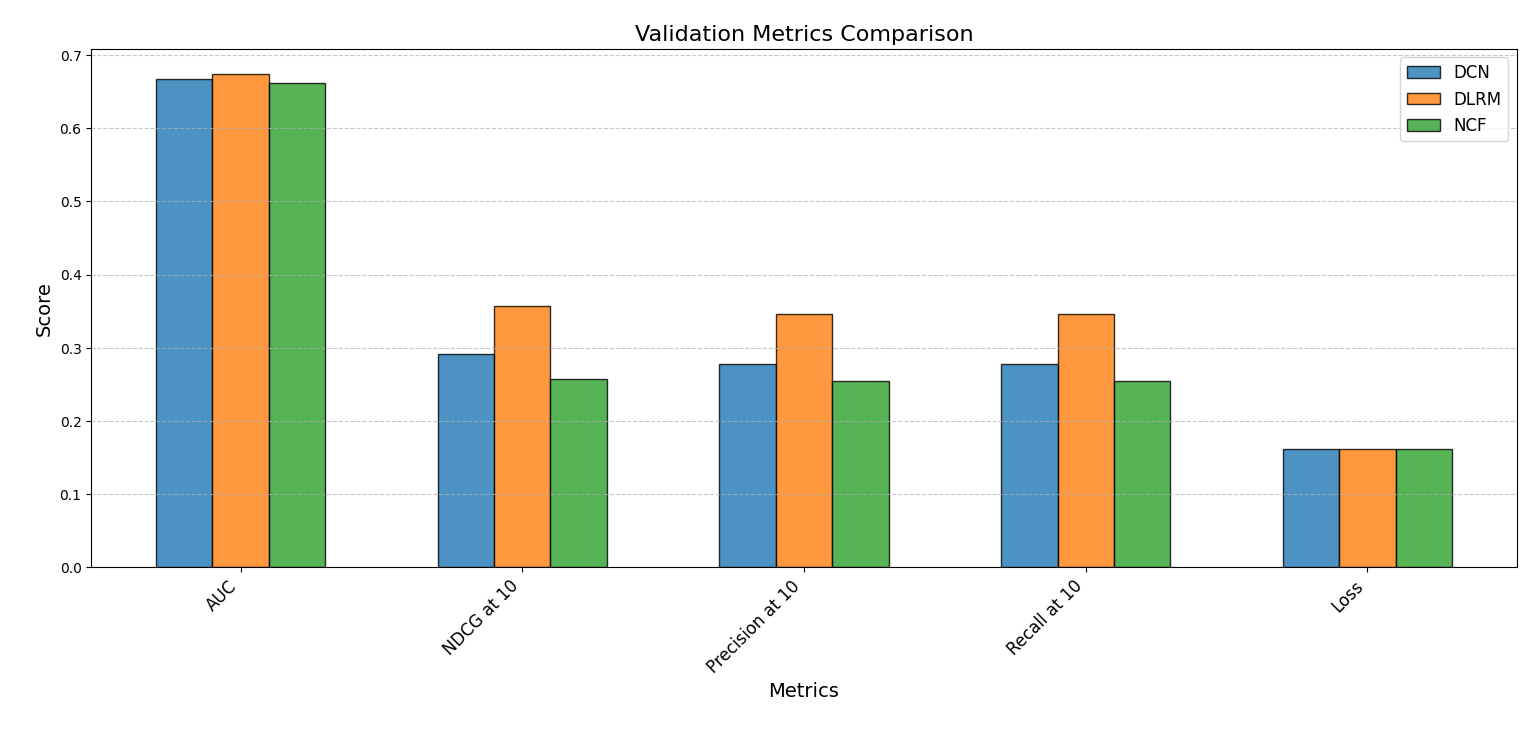
\includegraphics[width=\textwidth]{assets/Validation Metrics Comparison.png}
%     \caption[AUC Comparison]{AUC Comparison}
%     \label{fig:AUCComparison}
% \end{figure}

% The results show that all the models had a similar performance with AUC values around 0.5, which indicates that the models performed similarly.

% Recommending relevant items from millions of possibilities is a significant challenge. 
% Since systems typically show dozens of items, even a single click signifies the success of the system.


